\section{The ATLAS Detector}
\label{sec:atlas}

In this section we will extend our focus to the ATLAS detector, the general purpose
particle detector located at Point 1 of the LHC ring (see Figure~\ref{fig:p1}).
Roughly cylindrical in shape, coaxial with the colliding proton beams,
the ATLAS detector is 44\,m long and 25\,m tall.
It is by far the largest such detector ever built and,
generally, is the largest and most complex device ever constructed.
Being general purpose in scope, the ATLAS detector is hermetic and has
nearly $4\pi$ radians of solid angle coverage around the $pp$ collision
point. 
Such detectors are commonly designed to have various subsystems --- \textit{sub-detectors} ---
which are dedicated for the identification of specific types of particles
and interactions.
They tend to be layered about the interaction point and cylindrically symmetric
since the $pp$ interactions taking place within the detector have no preferred
direction in the plane transverse to the direction in which the proton beams
are travelling.
A view of the ATLAS detector and its subdectors is provided by Figure~\ref{fig:atlas_cutaway}.
In the following we will briefly describe each subsystem in turn, describing
first the detectors located nearer to the $pp$ collision and proceeding outwards.

\subsection{The ATLAS Coordinate System}
\label{sec:atlas_coordinate_system}

The ATLAS detector uses a right-handed coordinate system with the origin located at
the geometric center of the detector.
The $x$-axis points to the center of the LHC ring, the $y$-axis points upwards
and away from the center of the Earth, and the $z$-axis is along the beam-pipe.
The side associated with positive (negative) $z$
is referred to as the `A' (`C') side of the detector.\footnote{`A' for `airport',
since this is the side pointing towards Geneva International Airport, and
`C' for either `Crozet' or `Charly's', depending on who you ask, since this is the side
pointing towards the town of Crozet and/or Charly's Pub in the town of Saint-Genis-Pouilly.}
Due to its cylindrical symmetry, ATLAS also uses the cylindrical coordinates, $(r,\phi)$,
with $\phi$ the azimuthal angle about the $z$-axis and having $\phi = 0$ along the positve $x$-axis.
The spherical polar angle, $\theta$, is defined with respect to the $z$-axis, having
$\theta = 0$ parallel to the beam-pipe and $\theta = \pi/2$ in the $xy$-plane transverse
to the beam-pipe.
The pseudorapidity, $\eta$, is commonly used when describing systems of particles or locations within
the detector and is defined as $\eta = - \ln \left[ \tan \left( \theta / 2 \right) \right ]$.
The relationship between psuedorapidity and polar angle is illustrated in Figure~\ref{fig:eta_desc}.
Large (small) values of $\eta$ correspond to the \textit{forward} (\textit{central}) region of the detector.
The rapidity, $y$, is related to $\eta$ in certain situations and is defined as $y = \frac{1}{2} \ln \left( (E+p_z) / (E-p_z) \right)$.
The pseudorapidity of a particle traversing the detector is equal to its rapidity of
the particle is massless or ultra-relativistic; otherwise, they are generally different.
The comparison between a particle's pseudorapidity and rapidity is illustrated in
Figure~\ref{fig:eta_desc}.
The coordinates used to describe systems of particles are typically described by their
four-momenta: $(p_x, p_y, p_z)$ or, equivalently, $(\pT, \eta, \phi)$.
A distance metric commonly used to describe the distance between two systems of particles
in the detector is $\Delta R = \sqrt{ (\Delta \eta)^2 + (\Delta \phi)^2 }$. The
$\Delta R$ quantity using $y$ instead of $\eta$ is also sometimes used and will be
indicated by $\Delta R_y$.



\begin{figure}[!htb]
    \begin{center}
        \raisebox{1.5cm}{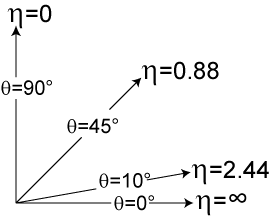
\includegraphics[width=0.35\textwidth]{figures/chapter2/eta_vs_polar}}
        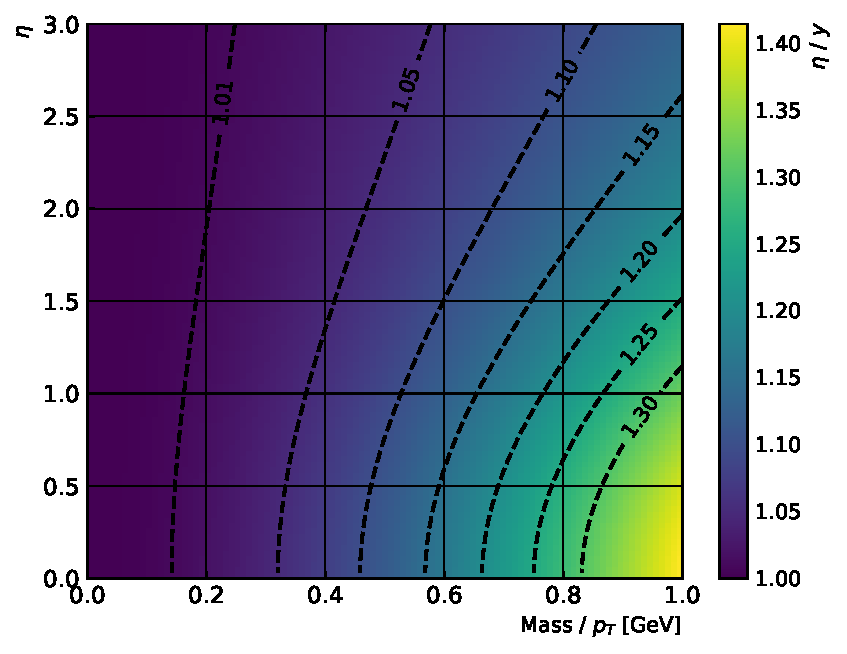
\includegraphics[width=0.55\textwidth]{figures/chapter2/eta_vs_rap}
        \caption{
            \textit{Left}: Illustration of the relationship between the pseudorapidity, $\eta$,
                and polar angle, $\theta$, defined as the angle with respect to the beam-axis ($z$-axis).
            \textit{Right}: Distribution of the ratio of a particle's pseudorapidity to its rapidity, $\eta$/$y$,
                as a function of its pseudorapidity ($y$-axis) and the ratio of its mass to its transverse momentum, \pT~($x$-axis).
        }
        \label{fig:eta_desc}
    \end{center}
\end{figure}


\begin{figure}[!htb]
    \begin{center}
        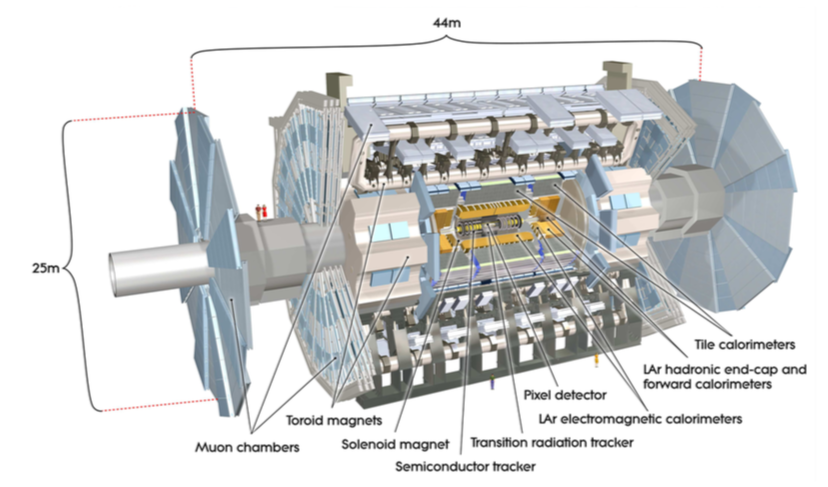
\includegraphics[width=0.95\textwidth]{figures/chapter2/atlas_cutaway}
        \caption{
            Cut-away view of the ATLAS detector with sub-systems indicated.
            Shown for comparison are figures of average-height humans standing
            at the feet of the detector and standing on the forward shielding
            between the big wheels of the forward muon system.
        }
        \label{fig:atlas_cutaway}
    \end{center}
\end{figure}


\begin{figure}[!htb]
    \begin{center}
        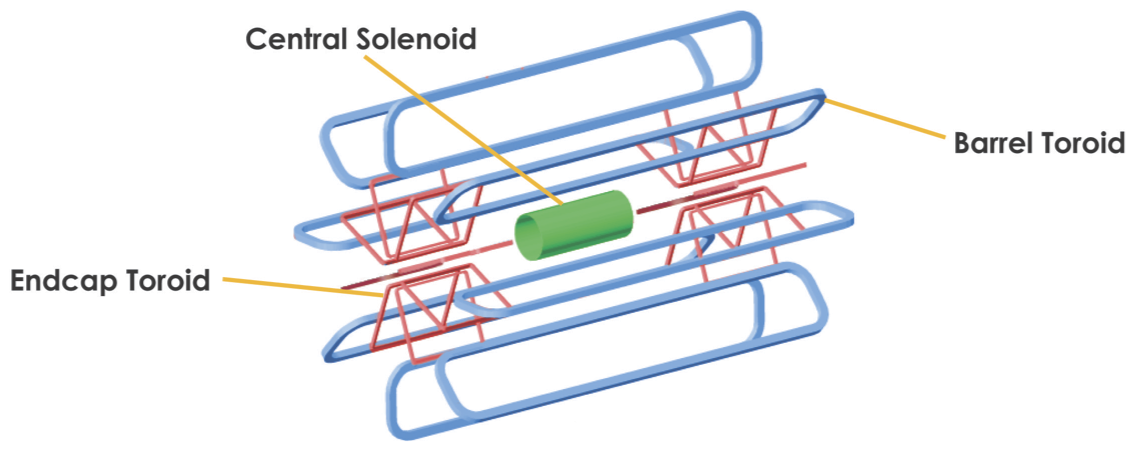
\includegraphics[width=0.95\textwidth]{figures/chapter2/atlas_magnet_system}
        \caption{
            A view of the ATLAS magnet system. Shown are the 2\,T solenoid magnet
            in green, the barrel toroid system in blue, and endcap toroid magnets
            in red.
        }
        \label{fig:atlas_magnet_system}
    \end{center}
\end{figure}
